\chapter{Runaway Ambipolar Diffusion in Protoplanetary Disks}
\label{1dvertical}





\section{Abstract}
We demonstrate that the magnetic field in the ambipolar damped region of a protoplanetary disk will exhibit runaway diffusion to a strongly magnetized state if the toroidal field is aligned in the same direction and exceeds a critical field strength.





\section{Introduction} 
Non-ideal MHD effects are relevant in protoplanetary disks, different effects in different places.  Ambipolar diffusion is dominant near the mid-plane of the disk for $r>10$ AU.  

Previous work shows that the primary result of this effect is to damp the MRI, thus the region around the mid-plane of the disk is often referred to as a "damping zone" or "dead zone".  

We demonstrate that, in addition to suppressing the MRI, ambipolar diffusion can become the dominant magnetic field transport mechanism near the mid-plane of the disk and cause the magnetic strength to increase drastically ("runaway diffusion").  This runaway is triggered when the toroidal field at the mid-plane is mostly aligned in the same direction and is above a critical value $\beta$ of the beta parameter. 

This paper is organized as follows: In section 3 we describe the 3D simulations in which this effect was first seen and briefly describe the underlying cause.  In section 4 we describe a 1D model developed to confirm our results and test various parameters.  In section 5 we present the results of this modeling.  In section 6 we summarize and discuss our main conclusions.  





\newpage
\section{3d Simulations}
This phenomena was first seen in a 3D non-ideal MHD simulation in a shearing box.


\subsection{Methods and Algorithm}
We use athena.


\subsection{Parameters and Setup}
Describe the physics we have on and parameters.  Probably plot Am. Explain where Am profile comes from.


\subsection{Results}
%\begin{figure}[h!]
%centering
%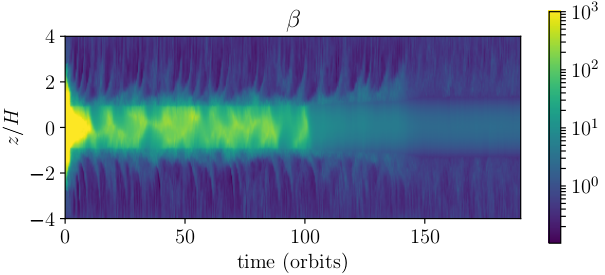
\includegraphics[width=0.49\columnwidth]{figs/figsChapter5/Beta_st.png}
%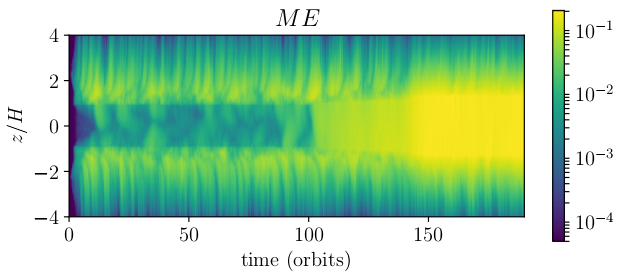
\includegraphics[width=0.49\columnwidth]{figs/figsChapter5/ME_st.png}
%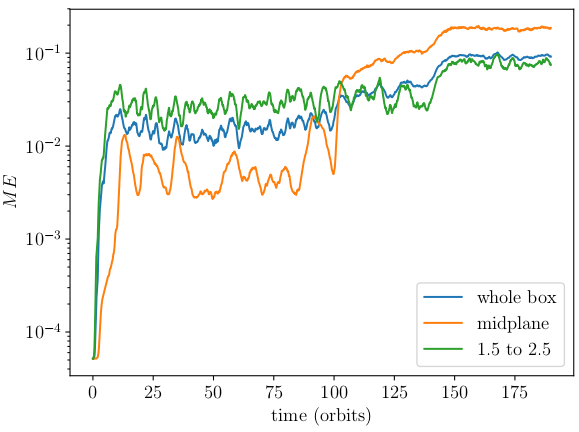
\includegraphics[width=0.44\columnwidth]{figs/figsChapter5/ME_vs_time.png}
%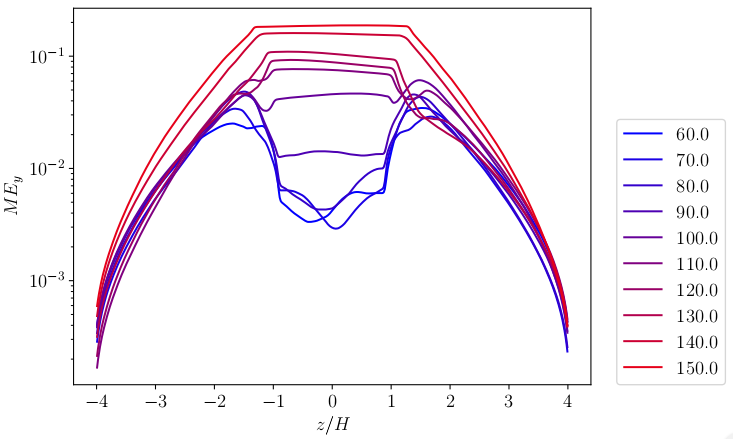
\includegraphics[width=0.55\columnwidth]{figs/figsChapter5/MEy_profile.png}
%\caption{Space-time diagrams for the $\beta$ parameter and the Magnetic Energy.  Runaway diffusion happens between 100 and 150 orbits.  NOTE: Need to plot By ST diagram here too or instead of ME.  Maybe also plot stress and that large scale / small scale stress comparison metric?}
%\label{3dPlots}
%\end{figure}

As seen in figure \ref{3dPlots}, the typical behaviour of the MRI is to build up toroidal field in either the positive or negative direction, with that direction changing in a quasi-periodic fashion.  Also, the MRI operates largely independently on either side of the damping zone.  As the field generated by the MRI is turbulently diffused into the damping zone, the net-field in the damping zone does something like a random walk.  

This typical behaviour holds true until around orbit 100, where the disk undergoes a transition.  The field at the mid-plane becomes 1-2 orders of magnitude stronger and the MRI on either side of the damping zone stops it's typical sign flipping behaviour and stays in the same direction for the duration of the simulation.

This dramatic change in the magnetic field configuration has several immediately evident effects.  First, the magnetic pressure gradient now contributes significantly to hydrostatic balance, causing the density and pressure profiles to flatten and causing the FUV ionization transition to move to higher $|z|$.  Second, the magnetic stress in the mid-plane region increases by about 1 order of magnitude.  However, almost all of this stress is on large scales.  The field is actually more laminar than before, but the increase in field strength is more than enough to compensate for this, so we see more stress in the strong magnetic state.



\newpage
\subsection{Heuristic Explanation of Observed Phenomena}
We propose that this magnetic state transition occurs when the ambipolar diffusion time across the mid-plane region becomes sufficiently short on a relevant length-scale.  An expansion of the ambipolar diffusion term in the induction equation shows that the "diffusion-like" term looks like

\begin{equation}
\frac{\partial \bold{B}}{\partial t} = \frac{\bold{B}^2}{\Omega \rho \hspace{0.5mm} \text{Am}} \cdot \nabla^2 \bold{B}.
\end{equation}

\noindent NOTE: check that this prefactor works out, also define Am and beta, probably in a previous section.

\noindent This is different than simple diffusion because the diffusion coefficient depends on the quantity being diffused.  The ambipolar diffusion time is dependent on the field strength, given by 

\begin{equation}
t_\text{AD} = \frac{L^2 \Omega \rho \hspace{0.5mm} \text{Am}}{B^2}
\end{equation}

\noindent where L is the length scale of interest. Substituting $\rho=P/c_s^2$, $c_s^2=(h\Omega)^2$, and $B^2=P/\beta$ yields

\begin{equation}
\Omega t_\text{AD} = \bigg(\frac{L}{h}\bigg)^2 \beta \hspace{0.5mm} \text{Am}.
\end{equation}

\noindent Based on the simulation, it appears that the critical $\beta$ parameter for runaway is $\sim 10^2$.  At this field strength, the ambipolar diffusion time will be $100\Omega^{-1}$ at scale $h$.  While this is much longer than the dynamical time, it is on the order of the turbulent diffusion time or shorter.  We will further explore the interaction of these 2 time-scales in the next two sections with a 1D model.   


\subsection{Dependence on 3D Field Structure and Field Alignment}
The point at which runaway diffusion begins depends not only on the strength of toroidal field as described above, but also how it is aligned and it's spatial distribution.  To state the obvious, diffusion of a magnetic field is inherently different than diffusion of other quantities because magnetic field can be positive or negative.  Thus, we could arrive at situations in which the mid-plane has $<|B|>$ which should be large enough to trigger runaway diffusion based on the heuristic criteria in the previous section, but $|<B>|$ in the region could be very close to zero.  This situation will result in a quick recombination of field, and the rate of diffusion will decrease instead of runaway.  Therefore our criteria for runaway diffusion should be based on the true mean field $|<B>|$ over the region instead of the mean field strength $<|B|>$.        

%\begin{figure}[h!]
%\centering
%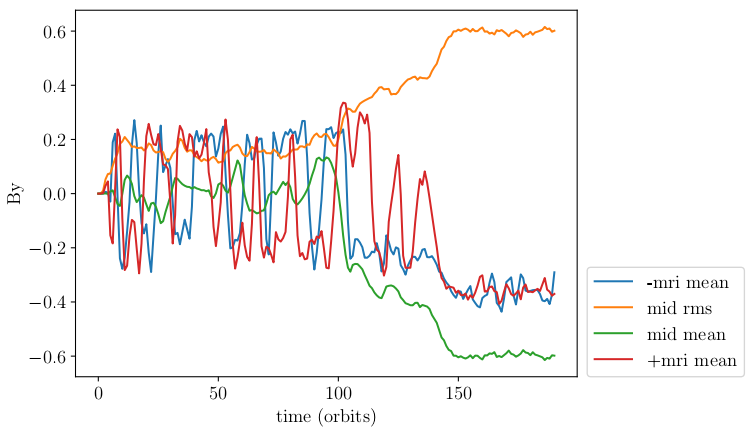
\includegraphics[width=0.5\columnwidth]{figs/figsChapter5/By_vs_time.png}
%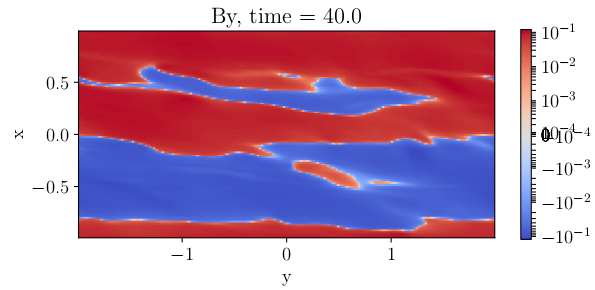
\includegraphics[width=0.5\columnwidth]{figs/figsChapter5/xyPlaneBy.png}
%\caption{NOTE: These figures are pretty sloppy right now, but something like this will get the point across.}
%\label{3dPlots}
%\end{figure}





\newpage
\section{Description of 1d Model}
To confirm that we are attributing this phenomenon to the correct physical processes and explore a range of parameters, we create a 1d toy model of the vertical profile of the magnetic field in a non-ideal disk.  This is also particularly useful because evolving systems with strong diffusion can be prohibitively computationally expensive in 3D.  


\subsection{Induction Equation Approximation}
We will evolve the magnetic field under the influence of an $\alpha$-parameterization of turbulent diffusion and an approximation of ambipolar diffusion.  

With these parameterizations, the induction equation is given by:

\begin{equation}
\frac{\partial B}{\partial t} = (\eta_{\text{AD}} + \eta_{\text{turb}}) \frac{\partial^2 B}{\partial z^2}.  \end{equation}

\noindent where the resistivities are given by:

\begin{equation}
\eta_{\text{turb}} = \frac{\alpha c_s h}{\text{Pr}},
\end{equation}
\begin{equation}
\eta_{\text{AD}}   = \frac{B^2}{\Omega \rho \hspace{0.5mm} \text{Am}}.                   
\end{equation}

\noindent We ignore the velocity terms under the assumption that there are no large scale (non-turbulent) motions in the vertical direction.  Note that $\eta_{\text{AD}}$ is a function of the quantity being diffused ($B$), and will be evolved self consistently as the field evolves.  


\subsection{Hydrostatic Equilibrium}
The disk is stratified according to hydrostatic equilibrium.  We will consider an isothermal disk.  Our model will consider 2 zones with different diffusion coefficients: mid-plane and corona.  The point at which the transition between these 2 zones occurs where the surface density (integrated outside-in) is equal to $\Sigma_\text{FUV}$.  We will call this point $z_\text{trans}$ and it will be evolved self-consistently.  
%The density is evolved to maintain this hydrostatic equilibrium as the magnetic field changes (contributing to the magnetic pressure term in the force balance equation). 


\subsection{Modeling the MRI and Buoyant Field Removal}
We will use very simple prescriptions to model the MRI and buoyant field removal.  The MRI is expected to build up field until a point of saturation at $\beta=\beta_\text{sat}$.  We will set $\beta_\text{sat}=3$ usually, as this is where the field becomes too strong for the MRI to operate because it is a weak field instability.  We will have the field approach this value with a characteristic $e$-folding time of $t_{\text{MRI}}$.  Where $|z|>z_{\text{trans}}$ and $\beta>\beta_{\text{sat}}$, the field evolution equation will also include this term:

\begin{equation}
\frac{\partial B}{\partial t} = \frac{B_{\text{sat}}-B}{t_\text{MRI}}, 
\end{equation}

\noindent where $B_{\text{sat}}$ is the field strength corresponding to $\beta_{\text{sat}}$.  

We will consider two cases: 1) The MRI only produces positive field.  2) The MRI can produce positive or negative field with the direction switching in a quasi-periodic manner independently on either side of the damping zone.  For the first case, $B_{\text{sat}}$ is constant in time.  For the second case, $B_{\text{sat}}$ can be positive or negative and will flip stochastically with a characteristic flip time of $1/t_{\text{flip}}$.  The MRI on the positive and negative sides of the box are assumed to operate independently of one another.  

We will model buoyant field removal from the upper corona in a similar way.  For the region $|z|>3H$, the field evolution equation will include the following term:

\begin{equation}
\frac{\partial B}{\partial t} = -\frac{B}{t_\text{buoyancy}}.
\end{equation}


\subsection{Summary of Parameter Choices}
Here we list our standard parameters.  Any changes or varied parameters will be specified with the results in the next section.  The ambipolar damped mid-plane region has $\text{Am}=1$ and $\alpha=10^{-4}$.  The MRI active corona has $\text{Am}=10^6$ and $\alpha=10^{-2}$.  In the corona, the MRI will cause the magnetic field to evolve towards a saturated state with $\beta_{\text{sat}}=3$ with a relaxation time of $t_\text{MRI}=2\pi \Omega^{-1}$.  Field is removed above $|z|=3$ with an $e$-folding time of $t_\text{buoyancy}=2\pi \Omega^{-1}$.  We will work in units where $H$ and $c_s$ =1.  We will take $\text{Pr}=1$.  


\subsection{Time Evolution Scheme and Summary of Model}
The time evolution scheme is done in a Runge-Kutta 4th order fashion with an adaptive time-step that follows a diffusive CFL condition.  To summarize:

\begin{enumerate}
\item{Initialize with a constant field throughout the disk, set such that $\beta=10^6$ at the mid-plane. }
\item{Calculate the density profile by applying hydrostatic equilibrium and including the magnetic pressure term.}
\item{Calculate the mid-plane corona transition point $z_{\text{trans}}$ from the density profile. }
\item{Calculate the diffusion coefficients $\eta_{\text{turb}}$ and $\eta_{\text{AD}}$ based on the density profile and $z_{\text{trans}}$.}
\item{Calculate dt based on the diffusion coefficients.}
\item{Use RK 4th order to evolve the magnetic field forward in time according to the induction equation.}
\item{Apply the MRI and buoyant field removal terms.}
\item{Repeat steps 2-7.}
\end{enumerate}





\newpage
\section{Results of 1D Modeling}
We will use our model to demonstrate that a disk with an MRI active corona will slowly diffuse some field towards the mid-plane through turbulence until the field reaches a critical value where ambipolar diffusion becomes dominant and diffuses field across the mid-plane much more quickly.


\subsection{Comparing Ambipolar Diffusion and Turbulent Diffusion}
The ratio of ambipolar diffusion to turbulent diffusion is given by

\begin{equation}
\frac{\eta_{\text{AD}}}{\eta_{\text{turb}}} = \frac{\text{Pr} \hspace{0.5mm} B^2}{\alpha c_s h \Omega \rho \hspace{0.5mm} \text{Am}}.
\end{equation}

\noindent $c_s$, $h$, and $\Omega$ are not functions of time or z.  We will work in units such that all of these quantities are 1.  We assume that the Prandtl number Pr is 1.  In this case, the ratio reduces to

\begin{equation}
\frac{\eta_{\text{AD}}}{\eta_{\text{turb}}} = \frac{1}{\beta \alpha \hspace{0.5mm} \text{Am}}.
\label{eqEtaRatio}
\end{equation}

\noindent  To phrase this equation differently, ambipolar diffusion will be stronger than turbulent diffusion if $\beta < \alpha \hspace{0.5mm} \text{Am}$.  If $\alpha=10^{-4}$ and $\text{Am}=1$ in the mid-plane region, then ambipolar diffusion will be stronger than turbulent diffusion if $\beta<10^4$.


\subsection{Constant MRI}
First we will consider the simpler case in which the MRI only generates field in the positive toroidal direction and does not change alignment.  Figure \ref{1dModelConstant} demonstrates that ambipolar diffusion is able to transport a large amount of field to the mid-plane much faster than turbulence alone.  The final state that is reached is very similar to that seen in the 3D simulation.  The field strength in the damping zone is set by the field strength at the edge of the damping zone, which primarily is set by $\beta_\text{sat}$.  

%\begin{figure}[h!]
%\centering
%\includegraphics[width=0.49\columnwidth]{figs/figsChapter5/noSC_noAD_constantMRI/B.png}
%\includegraphics[width=0.49\columnwidth]{figs/figsChapter5/noSC_AD_constantMRI/B.png}
%\includegraphics[width=0.49\columnwidth]{figs/figsChapter5/noSC_noAD_constantMRI/beta.png}
%\includegraphics[width=0.49\columnwidth]{figs/figsChapter5/noSC_AD_constantMRI/beta.png}
%\caption{Time evolution of the magnetic field strength for two cases: only turbulent diffusion (left) and both turbulent and ambipolar diffusion (right).  Field strength is shown in the top row and the $\beta$ parameter on the bottom row.  The dashed black line in all plots corresponds to $\beta=\beta_\text{sat}=3$.  The vertical dashed black lines correspond to $z=z_{\text{trans}}$. }
%\label{1dModelConstant}
%\end{figure}

Figure \ref{etaRatio} shows that the primary field transport mechanism in the damping zone changes from turbulence to ambipolar diffusion as the system evolves.  The stronger the field gets the stronger ambipolar diffusion becomes, so after $\eta_\text{AD}/\eta_\text{turb}$ exceeds 1, a runaway effect is seen and the final state is reached quickly.  

%\begin{figure}[h!]
%\centering
%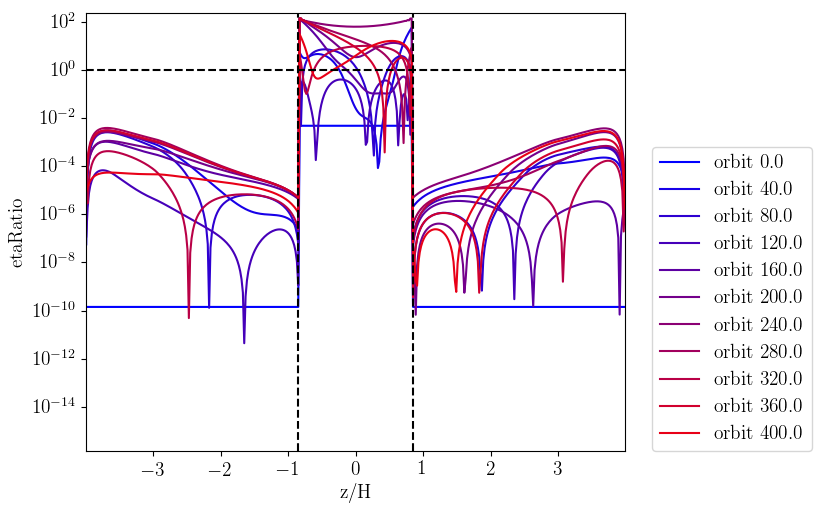
\includegraphics[width=0.49\columnwidth]{figs/figsChapter5/noSC_AD_constantMRI/etaRatio.%png}
%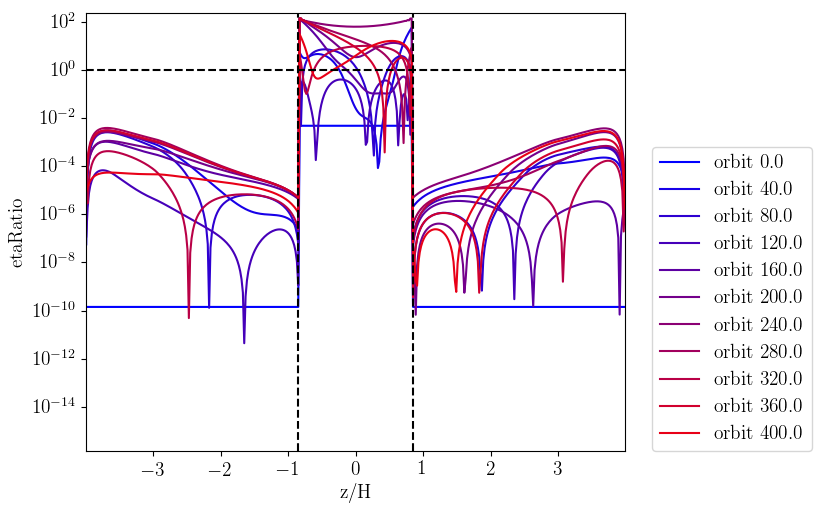
\includegraphics[width=0.49\columnwidth]{figs/figsChapter5/noSC_AD_constantMRI/etaRatio.png}
%\caption{The vertical profile of the ratio $\eta_\text{AD}/\eta_\text{turb}$ evolved over time.  NOTE: Second fig is a placeholder: should be looking at total eta profile or something.  }
%\label{etaRatio}
%\end{figure}

Based on equation \ref{eqEtaRatio}, $\beta$ and Am seem to be the most direct control parameters related to this phenomenon.  We will show how the steady state depends on value of Am in the damping zone and $\beta_{\text{sat}}$, the saturation level of the MRI.

The steady state value of $\eta_{\text{AD}}$ is set by the properties of the MRI and $\alpha$ in the corona.  We will define this to be $\eta_{\text{AD, SS}}$, and the associated steady state field strength $B_{\text{mid,SS}}$.  This field strength will be realized if the MRI is strong enough, i.e. $B_{\text{sat}}(z_\text{trans}) > B_{\text{mid,SS}}$.  If $B_{\text{sat}}(z_\text{trans}) < B_{\text{mid,SS}}$, then the mid-plane field strength will approach $B_{\text{sat}}(z_\text{trans})$.  So, somewhat counter-intuitively, stronger diffusion (smaller Am) leads to a weaker field at the mid-plane in the steady state.  

Figure \ref{betaAmRelation} demonstrates this effect.  Comparing the 3 plots in the top row, the field at the mid-plane approaches the same value regardless of the strength of the field in the corona.  

%\begin{figure}[h!]
%\centering
%\includegraphics[width=0.32\columnwidth]{figs/figsChapter5/betaMriTest/test_10/B.png}
%\includegraphics[width=0.32\columnwidth]{figs/figsChapter5/betaMriTest/test_11/B.png}
%\includegraphics[width=0.32\columnwidth]{figs/figsChapter5/betaMriTest/test_12/B.png}
%\includegraphics[width=0.32\columnwidth]{figs/figsChapter5/betaMriTest/test_0/B.png}
%\includegraphics[width=0.32\columnwidth]{figs/figsChapter5/betaMriTest/test_1/B.png}
%\includegraphics[width=0.32\columnwidth]{figs/figsChapter5/betaMriTest/test_2/B.png}
%\includegraphics[width=0.32\columnwidth]{figs/figsChapter5/betaMriTest/test_20/B.png}
%\includegraphics[width=0.32\columnwidth]{figs/figsChapter5/betaMriTest/test_21/B.png}
%\includegraphics[width=0.32\columnwidth]{figs/figsChapter5/betaMriTest/test_22/B.png}
%\caption{top to bottom: Am=0.1, 1, 10. \\
%left to right: $\beta_{\text{sat}}$=3, 30, 300.}
%\label{betaAmRelation}
%\end{figure}


%\begin{figure}[h!]
%\centering
%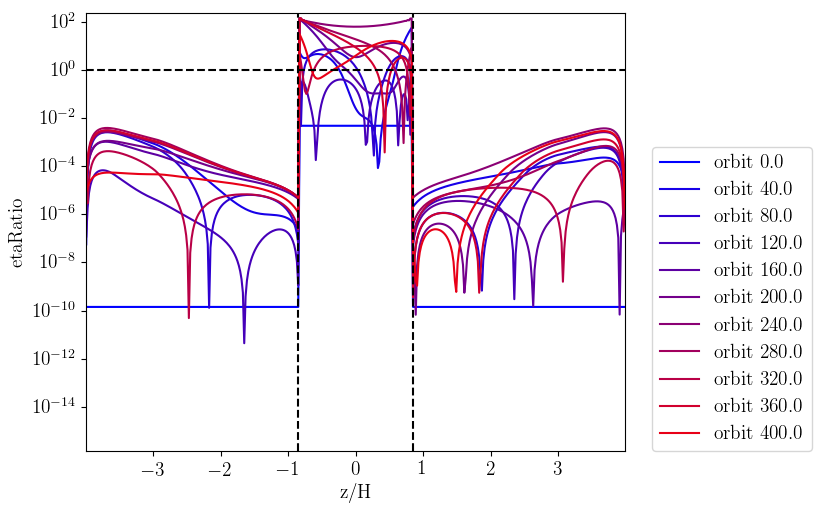
\includegraphics[width=0.49\columnwidth]{figs/figsChapter5/noSC_AD_constantMRI/etaRatio.png}
%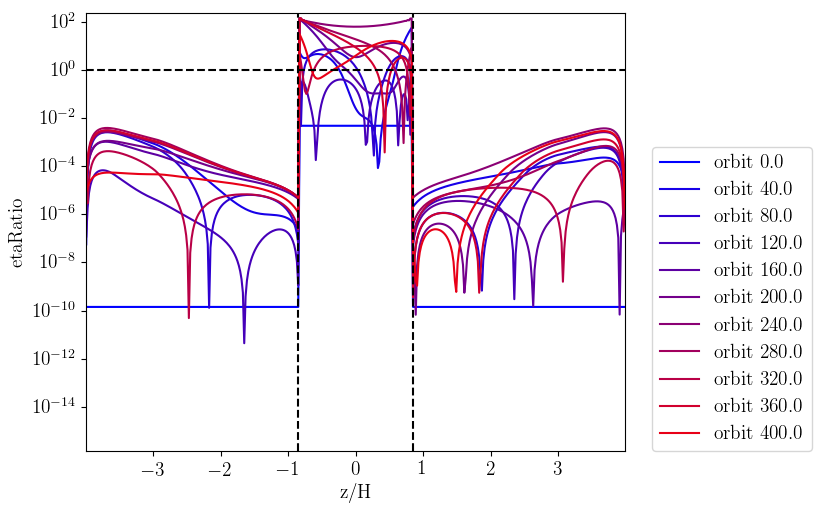
\includegraphics[width=0.49\columnwidth]{figs/figsChapter5/noSC_AD_constantMRI/etaRatio.png}
%\caption{NOTE: Placeholder for comparison to 3D data }
%\label{etaRatio}
%\end{figure}


\subsection{Quasi-Periodic MRI}
Here we will examine the results of the quasi-periodic MRI modeling.  

%\begin{figure}[h!]
%\centering
%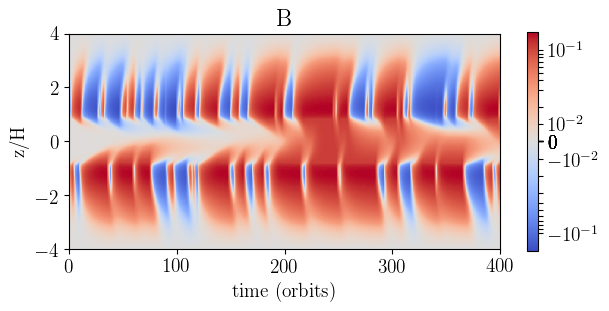
\includegraphics[width=0.6\columnwidth]{figs/figsChapter5/noSC_AD_randomMRI/B_ST2.png}
%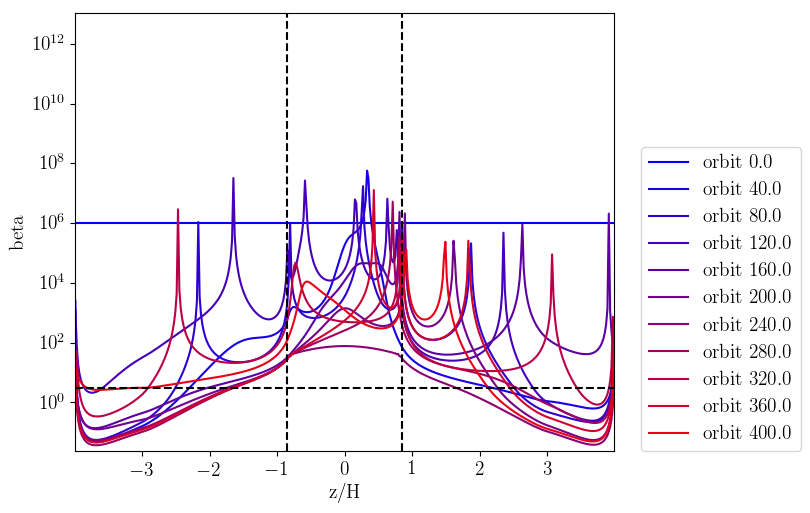
\includegraphics[width=0.8\columnwidth]{figs/figsChapter5/noSC_AD_randomMRI/beta.png}
%\caption{ }
%\label{1dModel}
%\end{figure}





\newpage
\section{Comparing the 1D model to 3D simulation data}





\newpage
\section{Conclusions and Discussion}
We conclude that the MRI in a protoplanetary disk is able to produce a strong enough toroidal magnetic field to cause ambipolar diffusion to dominate over turbulent diffusion around the mid-plane.  At this point, the magnetic field configuration of the disk changes dramatically: the mid-plane becomes rather strongly magnetized ($\beta \sim 10$ to $100$) and the MRI dynamo stops changing directions.

This magnetic state transition has several 

NOTE: Possible implications for: wind launching? (Bai 2013), 





%\newpage
%\section{Temporary Figures}
%\begin{figure}[h!]
%\centering
%\includegraphics[width=0.32\columnwidth]{figs/figsChapter5/betaMriTest/test_30/B.png}
%\includegraphics[width=0.32\columnwidth]{figs/figsChapter5/betaMriTest/test_31/B.png}
%\includegraphics[width=0.32\columnwidth]{figs/figsChapter5/betaMriTest/test_32/B.png}
%\includegraphics[width=0.32\columnwidth]{figs/figsChapter5/betaMriTest/test_10/B.png}
%\includegraphics[width=0.32\columnwidth]{figs/figsChapter5/betaMriTest/test_11/B.png}
%\includegraphics[width=0.32\columnwidth]{figs/figsChapter5/betaMriTest/test_12/B.png}
%\includegraphics[width=0.32\columnwidth]{figs/figsChapter5/betaMriTest/test_0/B.png}
%\includegraphics[width=0.32\columnwidth]{figs/figsChapter5/betaMriTest/test_1/B.png}
%\includegraphics[width=0.32\columnwidth]{figs/figsChapter5/betaMriTest/test_2/B.png}
%\includegraphics[width=0.32\columnwidth]{figs/figsChapter5/betaMriTest/test_20/B.png}
%\includegraphics[width=0.32\columnwidth]{figs/figsChapter5/betaMriTest/test_21/B.png}
%\includegraphics[width=0.32\columnwidth]{figs/figsChapter5/betaMriTest/test_22/B.png}
%\caption{top to bottom: Am=0.01, 0.1, 1, 10. \\
%left to right: betaSat=3, 30, 300.
%}
%\end{figure}


%\newpage
%\begin{figure}[h!]
%\centering
%\includegraphics[width=0.32\columnwidth]{figs/figsChapter5/betaMriTest/test_30/etaAd.png}
%\includegraphics[width=0.32\columnwidth]{figs/figsChapter5/betaMriTest/test_31/etaAd.png}
%\includegraphics[width=0.32\columnwidth]{figs/figsChapter5/betaMriTest/test_32/etaAd.png}
%\includegraphics[width=0.32\columnwidth]{figs/figsChapter5/betaMriTest/test_10/etaAd.png}
%\includegraphics[width=0.32\columnwidth]{figs/figsChapter5/betaMriTest/test_11/etaAd.png}
%\includegraphics[width=0.32\columnwidth]{figs/figsChapter5/betaMriTest/test_12/etaAd.png}
%\includegraphics[width=0.32\columnwidth]{figs/figsChapter5/betaMriTest/test_0/etaAd.png}
%\includegraphics[width=0.32\columnwidth]{figs/figsChapter5/betaMriTest/test_1/etaAd.png}
%\includegraphics[width=0.32\columnwidth]{figs/figsChapter5/betaMriTest/test_2/etaAd.png}
%\includegraphics[width=0.32\columnwidth]{figs/figsChapter5/betaMriTest/test_20/etaAd.png}
%\includegraphics[width=0.32\columnwidth]{figs/figsChapter5/betaMriTest/test_21/etaAd.png}
%\includegraphics[width=0.32\columnwidth]{figs/figsChapter5/betaMriTest/test_22/etaAd.png}
%\caption{top to bottom: Am=0.01, 0.1, 1, 10. \\
%left to right: betaSat=3, 30, 300.
%}
%\end{figure}


%\newpage
%\begin{figure}[h!]
%\centering
%\includegraphics[width=0.32\columnwidth]{figs/figsChapter5/betaMriTest/test_30/beta.png}
%\includegraphics[width=0.32\columnwidth]{figs/figsChapter5/betaMriTest/test_31/beta.png}
%\includegraphics[width=0.32\columnwidth]{figs/figsChapter5/betaMriTest/test_32/beta.png}
%\includegraphics[width=0.32\columnwidth]{figs/figsChapter5/betaMriTest/test_10/beta.png}
%\includegraphics[width=0.32\columnwidth]{figs/figsChapter5/betaMriTest/test_11/beta.png}
%\includegraphics[width=0.32\columnwidth]{figs/figsChapter5/betaMriTest/test_12/beta.png}
%\includegraphics[width=0.32\columnwidth]{figs/figsChapter5/betaMriTest/test_0/beta.png}
%\includegraphics[width=0.32\columnwidth]{figs/figsChapter5/betaMriTest/test_1/beta.png}
%\includegraphics[width=0.32\columnwidth]{figs/figsChapter5/betaMriTest/test_2/beta.png}
%\includegraphics[width=0.32\columnwidth]{figs/figsChapter5/betaMriTest/test_20/beta.png}
%\includegraphics[width=0.32\columnwidth]{figs/figsChapter5/betaMriTest/test_21/beta.png}
%\includegraphics[width=0.32\columnwidth]{figs/figsChapter5/betaMriTest/test_22/beta.png}
%\caption{top to bottom: Am=0.01, 0.1, 1, 10. \\
%left to right: betaSat=3, 30, 300.
%}
%\end{figure}